\documentclass{article}
\usepackage{booktabs}
\usepackage{graphicx}
\usepackage{hyperref}
\usepackage{amsmath}
\usepackage{float}

\title{Biol 461 Winter 2021\\ Assignment 3}
\author{Due 11:59pm on February 3rd, 2021}
\date{}

\begin{document}

\maketitle

\section*{Instructions}
%This assignment is broken into three parts. 
%Part A consists of questions drawn from the lectures and readings assigned thus far in the course.
%Part B consists of questions concerning addiction, science funding, and policy making.
%Part C is a bit of a choose-your-own-adventure; choose and complete \textbf{one} of the two provided options.

Please submit by uploading a PDF copy of your solutions to the Canvas assignment. 
Failure to submit the homework in the correct way and in the correct format may result in deduction of points. 
Incorrect solutions that do not show work will not receive any partial credit, so show your work where appropriate.

Collaboration with classmates is encouraged; however, your solutions should reflect your own understanding and all explanations should be in your own words. 
Please make a note of who you worked with on which parts of this homework.

\section*{Part A (X pts)}

\subsection*{Problem 1 (x pts)}
You discover a new ligand gated ion channel! Using patch clamp, you measure that at resting membrane potential (which for this cell is -70mV), exposing this ion channel to the agonist carbochol causes a flow of current into the cell. You want to determine what ion or ions are passing through this channel.\\
\begin{enumerate}
    \item[A. ] Is the reversal potential of this ion channel more negative than the resting membrane potential, equal to the resting membrane potential, or more positive than the resting membrane potential? How do you know? (State more negative, equal, or more positive and explain in 1-2 sentences)
    \item[B. ] You voltage clamp the cell at 0mV and again expose the channel to carbochol. You see a flow of current into the cell that is smaller than the current you saw when the cell was at resting membrane potential. State whether the reversal potential of this ion channel more negative than zero, equal to zero, or more positive than zero and 1-2 sentences explaining how you know.
    \item[C. ] Is the reversal potential of this ion channel closer to 0mV or to -70mV? How do you know? (1-2 sentences)
    \item[D. ] You voltage clamp the cell at 60mV and expose the channel to carbochol. You see no current. What is the reversal potential of this ion channel?
    \item[E. ] You voltage clamp the cell at 80mV and expose the channel to carbochol. You see a flow of current out of the cell. State whether the reversal potential of this ion channel more negative than zero, equal to zero, or more positive than zero and 1-2 sentences explaining how you know.
    \item[F. ] What ion or ions is this channel likely permeable to?
\end{enumerate}


\subsection*{Problem 2 (x pts)}
\begin{enumerate}
\item[A. ] Label each image below as a coronal, sagittal, or horizontal slice.
\begin{figure}[H]
\centering
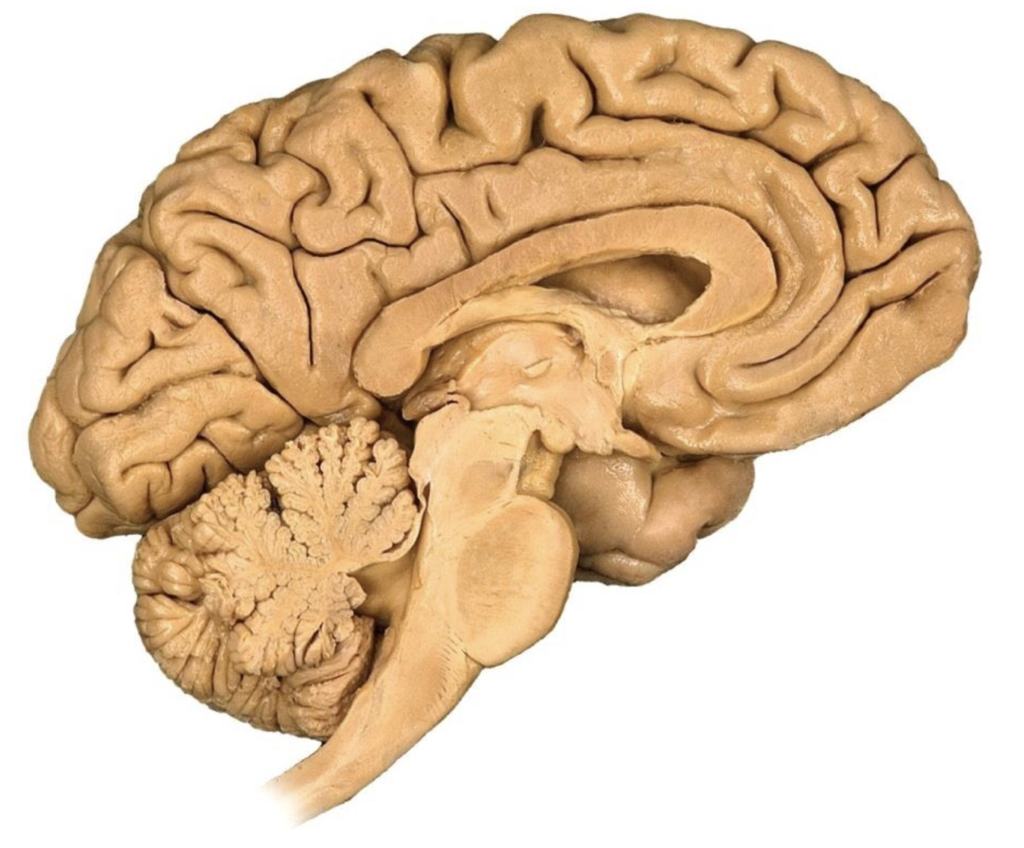
\includegraphics[width = .3\linewidth]{sagittal_slice.png}
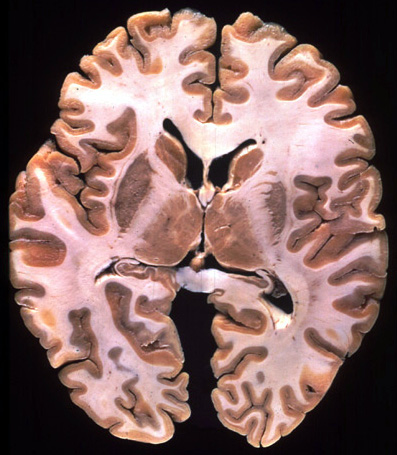
\includegraphics[width = .3\linewidth]{horizontal_slice.jpg}
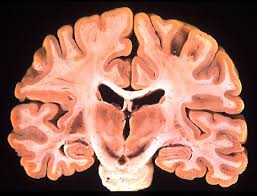
\includegraphics[width = .3\linewidth]{coronal_slice.jpeg}
\end{figure}
\vspace{5mm}
\item[B. ] Label which of the below nissl stained brain slices came from a human and which came from an eastern grey squirrel.
\begin{figure}[H]
\centering
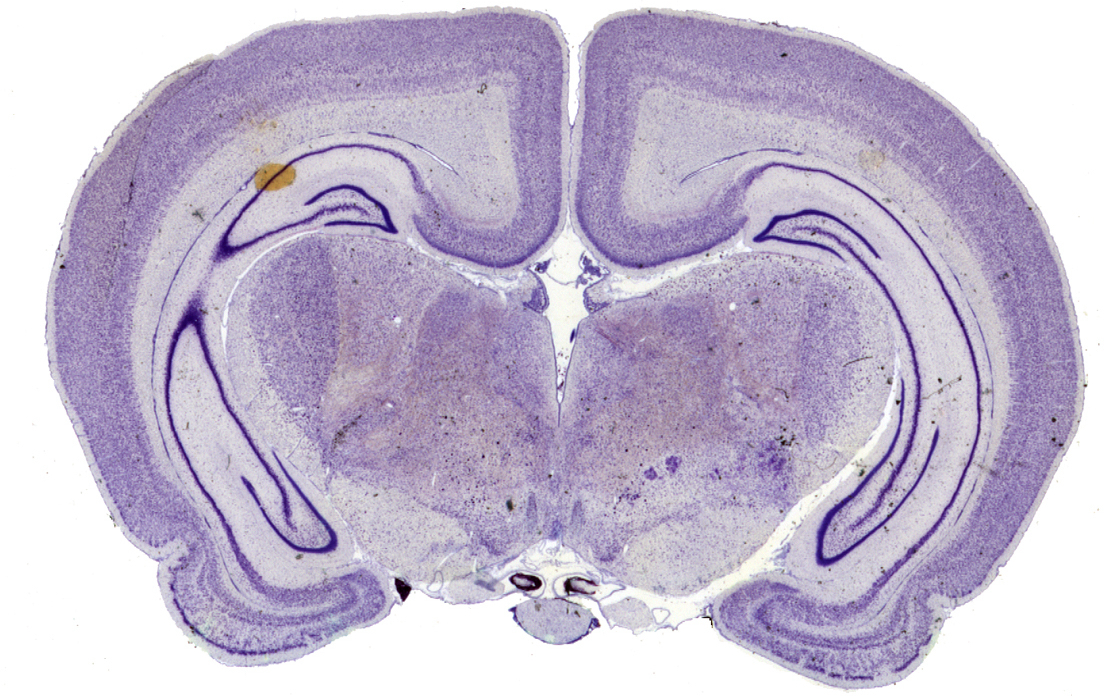
\includegraphics[width = .4\linewidth]{grey_squirrel_nissl_coronal.jpg}
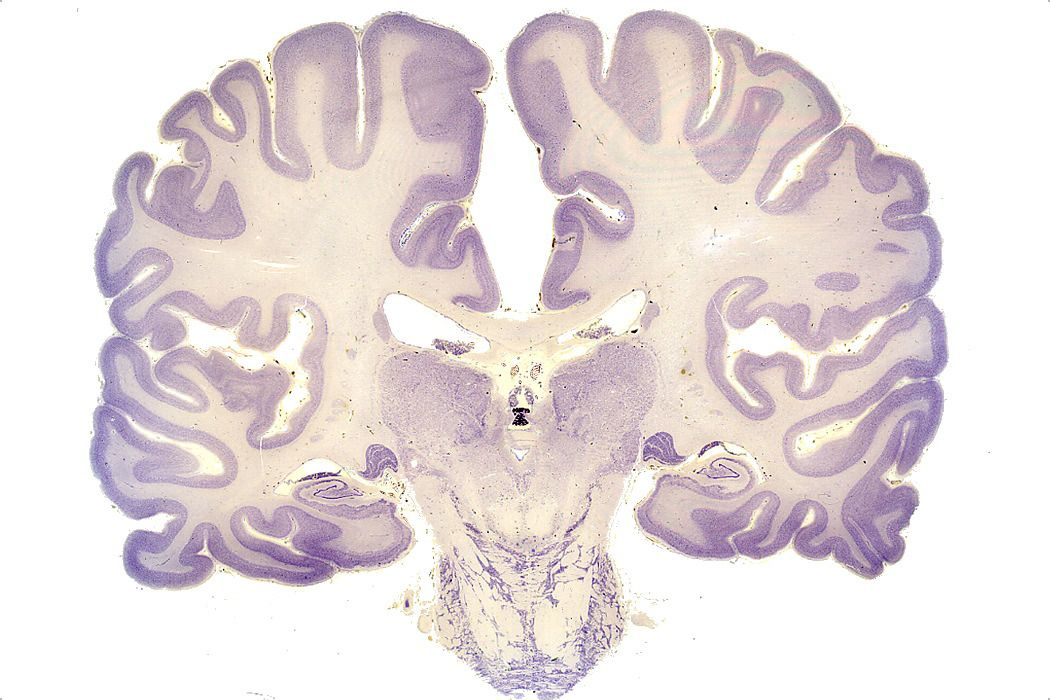
\includegraphics[width = .4\linewidth]{nissl_human_coronal.jpg}
\end{figure}
\vspace{5mm}
\end{enumerate}

\newpage
\subsection*{Part B, Choose your own adventure!  (X pts)}

Pick one of these paper to read, and then summarize the paper by answering the questions below.

\textbf{INSERT PAPER OR PAPERS}


\textbf{For the paper you chose}, in your own words, answer the following questions. (Each question is x pts) %each Q was 7 points last assignment


\begin{enumerate}

\item What are the major conclusions of the paper? In your own words, please summarize the major conclusions of the paper in 2--3 total sentences.

\item Why are these results significant? Specifically,  why should the scientific community care about these findings? Why should non-scientists care about these findings? ($\sim$2--3 sentences)

\item What were the key experimental or computational techniques the authors used? If more than one was used, how are the results interpreted together? ($\sim$2--3 sentences)

\item Pick one of the major results of the paper. What specific figures (e.g., ``Fig. 3b'' and ``Fig. 5a--c'')  show data to support this result? 
In your own words, summarize these data and how they support the result.  ($\sim$2--3 sentences)

\item Often, a paper is influential because it opens new avenues of future research. What new questions would you now ask having read this one? ($\sim$2-3 sentences)

\end{enumerate}


\end{document}
